\documentclass[12pt, a4paper, oneside, openright, titlepage]{book}
\usepackage[utf8]{inputenc}
\raggedbottom
\usepackage{import}


%%%%%%%%%%%%%%%%% Book Formatting Comments:

%%%%%%%%%%%%%%%%%%%%%%%%%%%%%%%%%%%%% for Part

%%%%%%%%%%%%%%%%%%%%%% for chapter

%%%%%%%%%%%%%%%%%%%% for section








%%%%%% PACKAGES %%%%%%%
\usepackage{hyperref}
\hypersetup{
    colorlinks,
    citecolor=black,
    filecolor=black,
    linkcolor=black,
    urlcolor=black
}
\usepackage{amsmath} % Math display options
\usepackage{amssymb} % Math symbols
\usepackage{amsfonts} % Math fonts
\usepackage{amsthm}
\usepackage{mathtools} % General math tools
\usepackage{array} % Allows you to write arrays
\usepackage{empheq} % For boxing equations
\usepackage{mathabx}
\usepackage{mathrsfs}
\usepackage{nameref}

\usepackage{soul}
\usepackage[normalem]{ulem}

\usepackage{txfonts}
\usepackage{cancel}
\usepackage[toc, page]{appendix}
\usepackage{titletoc,tocloft}
\setlength{\cftchapindent}{1em}
\setlength{\cftsecindent}{2em}
\setlength{\cftsubsecindent}{3em}
\setlength{\cftsubsubsecindent}{4em}
\usepackage{titlesec}

\titleformat{\section}
  {\normalfont\fontsize{25}{15}\bfseries}{\thesection}{1em}{}
\titleformat{\section}
  {\normalfont\fontsize{20}{15}\bfseries}{\thesubsection}{1em}{}
\setcounter{secnumdepth}{1}  
  
  

\newcommand\numberthis{\refstepcounter{equation}\tag{\theequation}} % For equation labelling
\usepackage[framemethod=tikz]{mdframed}

\usepackage{tikz} % For drawing commutative diagrams
\usetikzlibrary{cd}
\usetikzlibrary{calc}
\tikzset{every picture/.style={line width=0.75pt}} %set default line width to 0.75p

\usepackage{datetime}
\usepackage[margin=1in]{geometry}
\setlength{\parskip}{1em}
\usepackage{graphicx}
\usepackage{float}
\usepackage{fancyhdr}
\setlength{\headheight}{15pt} 
\pagestyle{fancy}
\lhead[\leftmark]{}
\rhead[]{\leftmark}

\usepackage{enumitem}

\usepackage{url}
\allowdisplaybreaks

%%%%%% ENVIRONMENTS %%%
\definecolor{purp}{rgb}{0.29, 0, 0.51}
\definecolor{bloo}{rgb}{0, 0.13, 0.80}



%%\newtheoremstyle{note}% hnamei
%{3pt}% hSpace above
%{3pt}% hSpace belowi
%{}% hBody fonti
%{}% hIndent amounti
%{\itshape}% hTheorem head fonti
%{:}% hPunctuation after theorem headi
%{.5em}% hSpace after theorem headi
%{}% hTheorem head spec (can be left empty, meaning ‘normal’)i


%%%%%%%%%%%%% THEOREM STYLES

\newtheoremstyle{BigTheorem}
{20pt}
{20pt}
{\slshape}
{}
{\Large\color{purp}\bfseries}
{.}
{\newline}
{\thmname{#1}\thmnumber{ #2}\thmnote{ (#3)}}



\newtheoremstyle{TheoremClassic}
{15pt}
{15pt}
{\slshape}
{}
{\bfseries}
{.}
{.5em}
{}

\newtheoremstyle{Definitions}
{15pt}
{15pt}
{\slshape}
{}
{\bfseries}
{.}
{.5em}
{\thmname{#1}\thmnumber{ #2}\thmnote{ (#3)}}


\newtheoremstyle{Remarks}
{10pt}
{10pt}
{\upshape}
{}
{\bfseries}
{.}
{.5em}
{}

\newtheoremstyle{Examples}
{10pt}
{10pt}
{\upshape}
{}
{\bfseries}
{.}
{.5em}
{}


%%%%%%%%%%%%% THEOREM DEFINITIONS

\theoremstyle{BigTheorem}
\newtheorem{namthm}{Theorem}
\newtheorem{conj}[namthm]{Conjecture}

\theoremstyle{TheoremClassic}
\newtheorem{thm}{Theorem}[section]
\newtheorem*{thm*}{Theorem}
\newtheorem{lem}[thm]{Lemma}
\newtheorem{cor}[thm]{Corollary}
\newtheorem{prop}[thm]{Proposition}
\newtheorem{claim}[thm]{Claim}


\theoremstyle{Definitions}
\newtheorem{defn}{Definition}[section]
\newtheorem{axi}[defn]{Axiom}
\newtheorem{cust}[defn]{}
\newtheorem{cons}[defn]{Construction}
\newtheorem{props}[defn]{Properties}
\newtheorem{proc}[defn]{Process}
\newtheorem*{law}{Law}


\theoremstyle{Examples}
\newtheorem{eg}{Example}[section]
\newtheorem{noneg}[eg]{Non-Example}
\newtheorem{xca}[eg]{Exercise}


\theoremstyle{Remarks}
\newtheorem{rmk}{Remark}[section]
\newtheorem{qst}[rmk]{Question}
\newtheorem*{ans}{Answer}
\newtheorem{obs}[rmk]{Observation}
\newtheorem{rec}[rmk]{Recall}
\newtheorem{summ}[rmk]{Summary}
\newtheorem{nota}[rmk]{Notation}
\newtheorem{note}[rmk]{Note}



\renewcommand{\qedsymbol}{$\blacksquare$}


\numberwithin{equation}{section}

\newenvironment{qest}{
    \begin{center}
        \em
    }
    {
    \end{center}
    }

%%%%%% MACROS %%%%%%%%%
%% New Commands
\newcommand{\ip}[1]{\langle#1\rangle} %%% Inner product
\newcommand{\abs}[1]{\lvert#1\rvert} %%% Modulus
\newcommand\diag{\operatorname{diag}} %%% diag matrix
\newcommand\tr{\mbox{tr}\.} %%% trace
\newcommand\C{\mathbb C} %%% Complex numbers
\newcommand\R{\mathbb R} %%% Real numbers
\newcommand\Z{\mathbb Z} %%% Integers
\newcommand\Q{\mathbb Q} %%% Rationals
\newcommand\N{\mathbb N} %%% Naturals
\newcommand\F{\mathbb F} %%% An arbitrary field
\newcommand\ste{\operatorname{St}} %%% Steinberg Representation
\newcommand\GL{\mathbf{GL}} %%% General Linear group
\newcommand\SL{\mathbf{SL}} %%% Special linear group
\newcommand\gl{\mathfrak{gl}} %%% General linear algebra
\newcommand\G{\mathbf{G}} %%% connected reductive group
\newcommand\g{\mathfrak{g}} %%% Lie algebra of G
\newcommand\Hbf{\mathbf{H}} %%% Theta fixed points of G
\newcommand\X{\mathbf{X}} %%% Symmetric space X
\newcommand{\catname}[1]{\normalfont\textbf{#1}}
\newcommand{\Set}{\catname{Set}} %%% Category set
\newcommand{\Grp}{\catname{Grp}} %%% Category group
\newcommand{\Rmod}{\catname{R-Mod}} %%% Category r-modules
\newcommand{\Mon}{\catname{Mon}} %%% Category monoid
\newcommand{\Ring}{\catname{Ring}} %%% Category ring
\newcommand{\Topp}{\catname{Top}} %%% Category Topological spaces
\newcommand{\Vect}{\catname{Vect}_{k}} %%% category vector spaces'
\newcommand\Hom{\mathbf{Hom}} %%% Arrows

\newcommand{\map}[2]{\begin{array}{c} #1 \\ #2 \end{array}}

\newcommand{\Emph}[1]{\textbf{\ul{\emph{#1}}}}

\newcommand{\mapsfrom}{\mathrel{\reflectbox{\ensuremath{\mapsto}}}}


%% Math operators
\DeclareMathOperator{\ran}{Im} %%% image
\DeclareMathOperator{\aut}{Aut} %%% Automorphisms
\DeclareMathOperator{\spn}{span} %%% span
\DeclareMathOperator{\ann}{Ann} %%% annihilator
\DeclareMathOperator{\rank}{rank} %%% Rank
\DeclareMathOperator{\ch}{char} %%% characteristic
\DeclareMathOperator{\ev}{\bf{ev}} %%% evaluation
\DeclareMathOperator{\sgn}{sign} %%% sign
\DeclareMathOperator{\id}{Id} %%% identity
\DeclareMathOperator{\supp}{Supp} %%% support
\DeclareMathOperator{\inn}{Inn} %%% Inner aut
\DeclareMathOperator{\en}{End} %%% Endomorphisms
\DeclareMathOperator{\sym}{Sym} %%% Group of symmetries


%% Diagram Environments
\iffalse
\begin{center}
    \begin{tikzpicture}[baseline= (a).base]
        \node[scale=1] (a) at (0,0){
          \begin{tikzcd}
           
          \end{tikzcd}
        };
    \end{tikzpicture}
\end{center}
\fi




\newdateformat{monthdayyeardate}{%
    \monthname[\THEMONTH]~\THEDAY, \THEYEAR}
%%%%%%%%%%%%%%%%%%%%%%%

%%% Specific Macros %%%


%%%%%% BEGIN %%%%%%%%%%


\begin{document}

%%%%%% TITLE PAGE %%%%%

\begin{titlepage}
    \centering
    \scshape
    \vspace*{\baselineskip}
    \rule{\textwidth}{1.6pt}\vspace*{-\baselineskip}\vspace*{2pt}
    \rule{\textwidth}{0.4pt}
    
    \vspace{0.75\baselineskip}
    
    {\LARGE Physics 375: Waves and Optics}
    
    \vspace{0.75\baselineskip}
    
    \rule{\textwidth}{0.4pt}\vspace*{-\baselineskip}\vspace{3.2pt}
    \rule{\textwidth}{1.6pt}
    
    \vspace{2\baselineskip}
    Phys 375 \\
    \vspace*{3\baselineskip}
    \monthdayyeardate\today \\
    \vspace*{5.0\baselineskip}
    
    {\scshape\Large E/Ea Thompson(they/them), \\ Physics and Math Honors\\}
    
    \vspace{1.0\baselineskip}
    \textit{Solo Pursuit of Learning}
    \vfill
    \enlargethispage{1in}
    \begin{figure}[b!]
    \makebox[\textwidth]{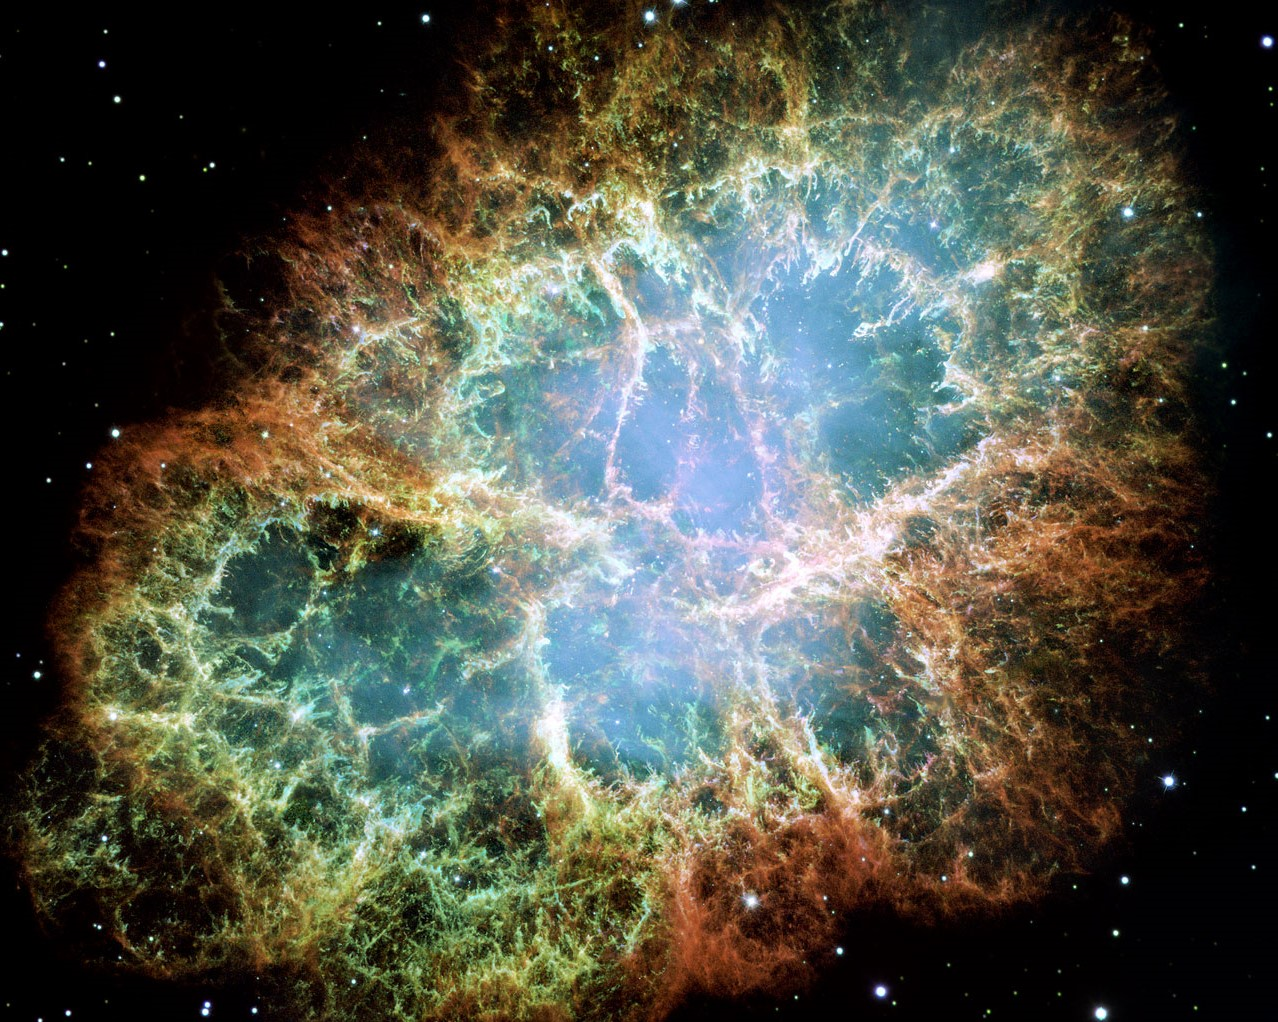
\includegraphics[width=\paperwidth, height =10cm]{../Crab.jpg}}
    \end{figure}
\end{titlepage}

%%%%%%%%%%%%%%%%%%%%%%%
\tableofcontents



%%%%%%%%%% Section 1 %%%%%%%%%%
\section{Review of Oscillations}

\subsection{Mass Spring System}

Consider a mass spring system with mass $M$ and a massless, frictionless spring of spring constant $k_s$. Letting $x = 0$ denote the equilibrium position of the mass spring system the force on the mass due to the spring, when located at a position $x$, is given by \textbf{Hooke's law}:
%%
\begin{equation}
    F = -k_sx
\end{equation}
%%
Note that this describes a restorative force, directed towards the equilibrium position of the mass spring system. We may also consider the length of the spring, $s$, in which case if the equilibrium length of the spring is $l$, Hooke's law may be expressed as 
%%
\begin{equation}
    F = k_s(l-s)
\end{equation}
%%
In general, a \textbf{restoring force} is a force acting on a system which seeks to return the system to some stable equilibrium state.


The oscillation frequency, $\nu$, for the mass spring system can be given by
%%
\begin{equation}
    \nu = \frac{1}{2\pi}\sqrt{\frac{k_s}{M}}\;\;(\text{cycles/sec}  = Hz)
\end{equation}
%%
Applying Newton's second law we can derive this expression through the equation of motion for the mass:
%%
\begin{equation}
    M\frac{d^2x}{dt^2} = -k_sx
\end{equation}
%%
Provided $k_s > 0$, this system has an oscillatory solution. If we consider the initial condition $x(0) = x_0$ and $\dot{x}(0) = v$, then
%%
\begin{equation}
    x(t) = x_0\cos(\omega t)+\frac{v}{\omega}\sin(\omega t)
\end{equation}
%%
where $\omega = \sqrt{\frac{k_s}{M}}$ is the angular frequency of the system, giving the previous frequency $\nu = \frac{\omega}{2\pi}$. 


Recall that the spring force is conservative (i.e. corresponds to an exact form), and so it has a potential function described by $F = -\nabla U$, which implies:
%%
\begin{equation}
    U = \frac{1}{2}k_sx^2
\end{equation}
%%


We can consider the oscillation in a mass spring system as being done by the energy, as potential energy is converted to kinetic and then back, with the total energy always being conserved since we are in an isolated system with a conservative force being the only force present.


\subsection{Other Mechanical Oscillation Systems}

Next let us consider a pendulum consisting of a massless string of length $l$ from its support, and a mass $M$ attached at the base of the string. The restoring force in this context is the gravitational force on the mass $M$. Explicitly, accounting for the constraining force for the string, the net restoring force when the mass is at an angle $\theta$ is:
%%
\begin{equation}
    F = -Mg\sin\theta
\end{equation}
%%
where we are using circular coordinates with the angle measured counter clockwise. Using the arc-length change of variables for the circular pendulum path, $x(t) = l\theta(t)$, the equation of motion can be written as 
%%
\begin{equation}
    Ml\frac{d^2\theta}{dt^2} = -Mg\sin(\theta)
\end{equation}
%%
Note this will indeed give an equation of motion independent of the mass $M$. However, since this is a \textbf{nonlinear differential equation} its solution is not as simple as the mass spring system. In fact, the solution cannot be expressed in a closed form. However, provided $|\theta| \ll 1\;rad$ we can Taylor expand $\sin\theta$ to obtain an approximate linear form of this system:
%%
\begin{equation}
    \frac{d^2\theta}{dt^2} \approx -\frac{g}{l}\theta
\end{equation}
%%
Thus, for small angles we obtain the approximate solution:
%%
\begin{equation}
    \theta(t) \approx \theta_0\cos(\omega t)+\frac{\dot{\theta}_0}{\omega}\sin(\omega t),\;\;\omega = \sqrt{\frac{g}{l}}
\end{equation}
%%

Next let us consider a balance wheel, such as in a watch, which oscillates about about its center with a spiral spring to provide a restoring torque. Let $I$ (kg$\cdot$m$^2$) denote the moment of inertia of the wheel. We can describe the restoring torque provided by the spring using $\tau = -k_\tau\theta$ where $k_\tau$ is the torsional constant and $\theta$ is the rotational angle of the wheel balance measured from the equilibrium (zero torsion) angular position.


Recall that the equation of motion for a rotational system such as this is given by:
%%
\begin{equation}
    I\frac{d^2\theta}{dt^2} = \tau=-k_\tau\theta
\end{equation}
%%
This again describes an oscillation, now with angular frequency:
%%
\begin{equation}
    \omega = \sqrt{\frac{k_\tau}{I}}
\end{equation}



\subsection{Electromagnetic Oscillation}

Oscillatory behaviour can be also found in circuits, such as an isolated $LC$ circuit, which will oscillate with angular frequency:
%%
\begin{equation}
    \omega = \frac{1}{\sqrt{LC}}
\end{equation}
%%
The energies oscillating in these systems are electric and magnetic potential energies stored in the capacitor and inductor, respectively.

Consider the scenario of a capacitor charged to a charge $q_0$ connected to an inductor of inductance $L$ with the closing of a switch. We can describe the voltage across the capacitor as:
%%
\begin{equation}
    V_C(t) = \frac{q(t)}{C}
\end{equation}
%%
while the potential across the inductor is described by
%%
\begin{equation}
    V_L(t) = -L\frac{dI(t)}{dt}
\end{equation}
%%
so by Kirchhoff's voltage law
%%
\begin{equation}
    L\frac{d^2q}{dt^2} = -\frac{q}{C}
\end{equation}
%%
where $I(t) = -\frac{dq(t)}{dt}$ when considering a discharging capacitor. This gives the angular frequency described previously.

Recall that the electric potential energy stored in a capacitor may be described as:
%%
\begin{equation}
    U_e = \frac{q^2(t)}{2C}
\end{equation}
%%
while the magnetic potential energy stored in an inductor is given by:
%%
\begin{equation}
    U_m = \frac{1}{2}LI^2(t)
\end{equation}


\subsection{Damped Oscillation}

Consider a capacitor $C$ with a charge $q_0$ which is connected to an inductor $L$ through a finite resistance $R$. Using Kirchhoff's voltage law we can again write:
%%
\begin{equation}
    \frac{q(t)}{C} - RI(t)-L\frac{dI(t)}{dt} = 0
\end{equation}
%%
Recalling $I(t) = -dq(t)/dt$, this becomes a second order linear differential equation with constant coefficients:
%%
\begin{equation}
    \frac{d^2q(t)}{dt^2}+\frac{R}{L}\frac{dq(t)}{dt}+\frac{1}{LC}q(t) = 0
\end{equation}
%%
We can solve this system using the method of the Laplace transform, but for the current study this is sufficient. In the case of weak damping, $R \ll \sqrt{\frac{2L}{C}}$, this system has an approximate solution:
%%
\begin{equation}
    q(t) = q_0e^{-\gamma t}\cos\omega t
\end{equation}
%%
where $\gamma = \frac{R}{2L}$ is the damping constant.




%%%%%%%%%%%%%%%%%%%%%%%%%%%%%
\section{Wave Motion}

Waves propagate through a certain medium or they move in space, while oscillations are localized at one point in space. The independent variables for waves are the spatial and temporal positions.


\subsection{Creation of Waves on a String}

Consider a horizontal string attached on one end to a vertical mass-spring system. As the mass oscillates, waves propagate along the string, with spatial period $\lambda$ proportional to the frequency of the mass-spring oscillations. The oscillating mass transfers energy and momentum into string.

If $\lambda \;(\text{m})$ is the spatial period, called the \textbf{wavelength}, and $\nu$ is the frequency, then the propagation speed of the wave is
%%
\begin{equation*}
    \nu\lambda = c_w
\end{equation*}
%%
The propagation velocity is the fundamental quantity to characterize waves and is determined by the physical constants of the wave medium. 

Note that waves do not have to be sinusoidal - this behaviour depends on the generator for the wave. However, using Fourier analysis all such wave patterns can be approximated via suitably large superpositions of sinusoidal waves.



\subsection{Sinusoidal (Harmonic) Waves}

Consider a sinusoidal wave with amplitude $A$, frequency $\nu$, and wavelength $\lambda$ propagating in the positive $x$ direction with velocity $c_w$. The wave propagation can be given by
%%
\begin{equation}
    A\sin\left(\frac{2\pi}{\lambda}(x-c_wt)\right)
\end{equation}
%%
We can also express this as the imaginary component of the complex exponential:
%%
\begin{equation}
    f_{sin}(x,t) = A\text{Im}\;\exp\left[i\frac{2\pi}{\lambda}(x-c_wt)\right]
\end{equation}
%%
where the amplitude is real valued. Since $\frac{2\pi}{\lambda}c_2 = 2\pi\nu = \omega$, we can write 
%%
\begin{equation}
    f(x,t) = A\sin\left(\frac{2\pi x}{\lambda}-\omega t\right)
\end{equation}
%%
Additionally, let $k = 2\pi/\lambda$, which we refer to as the \textbf{wavenumber} (although the actual number of waves in $1\;\text{m}$ is given by $1/\lambda$). We can then write
%%
\begin{equation}
    c_w = \nu\lambda = \frac{\omega}{k}
\end{equation}
%%


\subsection{Wave Differential Equation}

The wave (differential) equation is given by
%%
\begin{equation}
    \frac{\partial^2 f}{\partial t^2} = c_w^2\frac{\partial^2 f}{\partial x^2}
\end{equation}
%%

The quantity $\phi = kx-\omega t$ we have seen thus far is called the \textbf{phase}.


\subsection{Nonsinusoidal Waves}

A family of solutions to the wave equation are given by arbitrary $C^2$ functions $f$ which can be written as 
%%
\begin{equation}
    f(x,t) = f(x\pm c_wt)
\end{equation}
For example, we could have a Gaussian pulse
%%
\begin{equation}
    f(x-c_wt) = Ae^{-(x-c_wt)^2/a^2}
\end{equation}
%%
where $a$ determines the spatial width of the pulse.


The constancy of propagation velocity satisfied by such things as sound waves completely breaks down for water waves - it doesn't just depend on the medium, but also the waveform or wave frequency. This is also true of the velocity of light in different media such as glass, which depends on the wavelength of wave frequency of the light.


\subsection{Phase and Group Velocities, Dispersion}

Waves with constant propagation velocity are called \textbf{nondispersive} or \textbf{dispersionless}. If the propagation velocity depends on wave frequency, such waves are called dispersive. Nondispersive waves are described by our previously given wave equation. 

For dispersive waves the pulse initially created is severely deformed as it propagates.

The velocity defined by $\omega/k$ is called the \textbf{phase velocity}, while the velocity $d\omega/dk$ is called the \textbf{group velocity}. In dispersive waves these may be different. We may use this to define dispersive and nondispersive waves:
%%
\begin{align*}
    \text{Dispersive wave: }&\;\frac{d\omega}{dk}\neq \frac{\omega}{k} \\
    \text{Nondispersive wave: }&\;\frac{d\omega}{dk} = \frac{\omega}{k} = const.
\end{align*}
%%

\subsection{Superposition of Two Waves}

Consider two sinusoidal waves of equal amplitude $A$, but different frequencies $\omega_1,\omega_2$, both propagating in the positive $x$ direction. The sum of the two waves can be written using a trig identity as
%%
\begin{equation}
    f(x,t) = 2A\sin\left[\frac{(k_1+k_2)x-(\omega_1+\omega_2)t}{2}\right]\cos\left[\frac{(k_1-k_2)x-(\omega_1-\omega_2)t}{2}\right]
\end{equation}
%%
If we take the limit as $\omega_1-\omega_2\rightarrow 0$, we obtain a wave envelope with fine ripples given by the phase velocity $c_{ph} = \frac{\omega_1}{k_1}$, and the envelope given by the group velocity $c_g = \frac{d\omega}{dk}$.

Later, it will be shown that energy is transferred with the group velocity, rather than the phase velocity, making it a more fundamental quantity. 

The superposition of two waves of slightly different frequencies yields an important phenomenon called \textbf{beats}. The high-frequency oscillations, $\approx \omega_1$, have their amplitudes modulated by a slowly varying, $|\omega_1-\omega_2|\ll \omega_1$, sinusoidal function.




%%%%%%%%%%%%%%%%%%%%%%%%%%%%%%%%%%%%%%%%%%
\section{Mechanical Waves}

\begin{defn}
    \textbf{Mechanical waves} are thse that can be created and propagated in elastic material media (e.g. sound waves in gases, liquids, and solids, and waves on an elastic string). \textbf{Electromagnetic waves}, on the other hand, do not require any material media. However, electromagnetic waves can also propagate in material media.
\end{defn}

One key requirement for a medium to accommodate mechanical waves is that the medium be elastic (if it is compressed or expanded by a force, it should be able to restore its original shape when the force is removed). Elasticity and inertia (mass) are two major physical properties that determine the propagation velocity of mechanical waves. In a propagating wave without reflection, the kinetic energy and the potential energy are the same, while in oscillations they are mutually exclusive, and the sum of the two energies is a constant.


\subsection{Mass-Spring Transmission Line}

Consider a sequence of mass-springs each with spring constant $k_s$ and a mass $M$, and a rest length $\Delta x$ between each spring. Let $\xi(x)$ denote the displacement from equilibrium of the mass with equilibrium position $x$. What propagates with the disturbance (or wave) is energy. The force on the mass at $x$ due to the spring to the left of it is given by
%%
\begin{equation*}
    F_- = -k_s\left[\xi(x)-\xi(x-\Delta x)\right]
\end{equation*}
%%
while the spring to the right of the mass at $x$ exerts a force
%%
\begin{equation*}
    F_+ = k_s\left[\xi(x+\Delta x)-\xi(x)\right]
\end{equation*}
%%
Then the net force on the mass at $x$ is
%%
\begin{equation*}
    F = k_s\left[\xi(x+\Delta x)+\xi(x-\Delta x)-2\xi(x)\right]
\end{equation*}
%%
By Newton's second law we have that 
%%
\begin{equation*}
    M\frac{\partial^2\xi(x,t)}{\partial t^2} = k_s\left[\xi(x+\Delta x)+\xi(x-\Delta x)-2\xi(x)\right] \approx k_s(\Delta x)^2\frac{\partial^2\xi(x,t)}{\partial x^2}
\end{equation*}
%%
after Taylor expanding about zero for $\Delta x$ small. Our wave or propagation velocity is 
%%
\begin{equation*}
    c_w = \Delta x\sqrt{\frac{k_s}{M}} = \sqrt{\frac{k_s\Delta x}{M/\Delta x}} = \sqrt{\frac{K}{\rho_l}}
\end{equation*}
%%
where $K$ is the elastic modulus and $\rho_l$ is the linear mass density. This allows us to write
%%
\begin{equation*}
    F = k_s\Delta l = k_sl\frac{\Delta l}{l} = K\frac{\Delta l}{l}
\end{equation*}
%%



\subsection{Energy Carried by Waves}

If we differentiate the mechanical wave $\xi(x,t)$ we can obtain the \textbf{velocity wave}
%%
\begin{equation*}
    v(x,t) = \frac{\partial \xi}{\partial t}
\end{equation*}
%%
and the kinetic energy of the mass is given by
%%
\begin{equation*}
    KE = \frac{1}{2}M\left(\frac{\partial\xi}{\partial t}\right)^2
\end{equation*}
%%
and the potential energy is given by
%%
\begin{equation*}
    PE = \frac{1}{2}k_s\left(\Delta x\right)^2\left(\frac{\partial\xi}{\partial x}\right)^2 = \frac{1}{2}c_w^2M\left(\frac{\partial \xi}{\partial x}\right)^2
\end{equation*}
%%
Setting $X = x-c_wt$ we can see that the potential energy and the kinetic energy are the same everywhere and anytime. Then the total wave energy is
%%
\begin{equation*}
    TE = Mc_w^2\left(\frac{\partial\xi}{\partial x}\right)^2 = Mc_w^2\left(\frac{d\xi}{dX}\right)^2
\end{equation*}
%%
Dividing by the length $\Delta x$, the total energy per unit length is given by
%%
\begin{equation*}
    \frac{TE}{\Delta x} = \rho_lc_w^2\left(\frac{d\xi}{dX}\right)^2
\end{equation*}
%%
The average wave energy density is
%%
\begin{equation*}
    TE_{avg} = \frac{1}{2}\rho_l\omega^2\xi_0^2
\end{equation*}
%%
and the rate of energy transfer is given by multiplying by the propagation speed
%%
\begin{equation*}
    \text{rate }TE_{avg} = \frac{1}{2}c_2\rho_l\omega^2\xi_0^2
\end{equation*}
%%


\subsection{Momentum Carried by Waves}

Let $\rho_l$ be the mass density in the absence f the wave and $\Delta \rho_l$ be the change in mass density due to the wave. If we have a mass density of $\rho_l$ over a length $\Delta x$ originally, and the length is stretched/compressed by the displacements $\xi(x)$ and $\xi(x+\Delta x)$, the original length $\Delta x$ now becomes
%%
\begin{equation*}
    \Delta x+\xi(x+\Delta x)-\xi(x) \approx \Delta x+\frac{\partial\xi}{\partial x}\Delta x
\end{equation*}
%%
so
%%
\begin{equation*}
    (\rho_l+\Delta \rho_l)\left(\Delta x+\frac{\partial \xi}{\partial x}\Delta x\right) = \rho_1
\end{equation*}
%%
or
%%
\begin{equation*}
    \Delta \rho_l = -\rho_l\frac{\partial\xi/\partial x}{1+\partial \xi/\partial x} \approx -\rho_l\frac{\partial\xi}{\partial x}
\end{equation*}
%%
assuming $|\partial\xi/\partial x|\ll 1$. Then the momentum density wave is given by
%%
\begin{equation*}
    \rho_l\frac{\partial\xi}{\partial t}-\rho_l\frac{\partial \xi}{\partial t}\frac{\partial \xi}{\partial x}
\end{equation*}
%%
The average momentum density is given by the average energy density over the wave velocity. 



\subsection{Transverse Waves}


The velocity of waves on a string under a tension $T$ has the form
%%
\begin{equation*}
    c_w = \sqrt{\frac{T}{\rho_l}}
\end{equation*}
%%
where $\rho_l$ is the linear mass density of the string.

Consider a small segment of string, $\Delta x$, with mass $\rho_l\Delta x$. Let $\xi(x)$ and $\xi(x+\Delta x)$ denote the perpendicular displacement. The net vertical force on the string due to tension
%%
\begin{equation*}
    F = T\sin\theta_2 - T\sin\theta_1
\end{equation*}
%%
where $\theta_2$ and $\theta_1$ are the angles of the tangent lines at $A$ and $B$, respectively,
%%
\begin{equation*}
    \tan\theta_1 = \frac{\partial\xi}{\partial x}(x)
\end{equation*}
%%
and
%%
\begin{equation*}
    \tan\theta_2 = \frac{\partial\xi}{\partial x}(x+\Delta x)
\end{equation*}
%%
If the displacement $\xi(x,t)$ is small, so are the angles. Then we approximate
%%
\begin{equation*}
    F = T\left(\frac{\partial\xi}{\partial x}\Bigg\vert_{x+\Delta x}-\frac{\partial\xi}{\partial x}\Bigg\vert_x\right) \approx \Delta x T\frac{\partial^2\xi}{\partial x^2}
\end{equation*}
%%
This is the force that acts on the segment with the mass $\rho_l\Delta x$. Therefore, Newton's equation of motion gives
%%
\begin{equation*}
    \rho_l\Delta x\frac{\partial^2\xi}{\partial t^2} = \Delta x T\frac{\partial^2\xi}{\partial x^2}
\end{equation*}
%%
or
%%
\begin{equation*}
    \frac{\partial^2\xi}{\partial t^2} = \frac{T}{\rho_l}\frac{\partial^2\xi}{\partial x^2}
\end{equation*}
%%


As before, the energy transfer rate is
%%
\begin{equation*}
    \frac{TE}{\Delta t} = c_w\rho_l\left(\frac{\partial\xi}{\partial t}\right)^2
\end{equation*}
%%
and
\begin{equation*}
    \text{momentum transfer rate} = \frac{\text{energy transfer rate}}{c_w}
\end{equation*}
%%

Likewise,
%%
\begin{equation*}
    \text{momentum density} = \frac{\text{energy density}}{c_w}
\end{equation*}
%%


We then have
%%
\begin{equation*}
    -\rho_l \frac{\partial\xi}{\partial t}\frac{\partial\xi}{\partial x} = \frac{1}{c_w}T \left(\frac{\partial \xi}{\partial x}\right)^2
\end{equation*}
%%
where 
%%
\begin{equation*}
    -\rho_l\frac{\partial\xi}{\partial t}\frac{\partial \xi}{\partial x}
\end{equation*}
%%
is the wave momentum density.


















%%%%%%%%%%%%%%%%%%%%%%%%%%%%%%%%%%%%%%
\section{Interference and Diffraction}



A harmonic wave in typical form is given by $A\sin(kx-\omega t)$ which is characterized by the amplitude $A$, the angular frequency $\omega$, and the wavelength $\lambda = 2\pi/k$. We consider the superposition of a collection of waves, all of the same amplitude. 


\subsection{Interference between two harmonic waves}


Consider two point wave sources separated by a distance $d$, radiating waves at identical frequencies. Consider a point $P$ at which we place a wave detector. The distances between $P$ and the wave sources are $x_1$ and $x_2$, respectively. The field amplitudes at $P$ are proportional to $1/x_1$ and $1/x_2$, respectively, with phases $2\pi x_1/\lambda$ and $2\pi x_2/\lambda$, which are proportional to $x_1$ and $x_2$.


The amplitude difference may not be important if the  point $P$ is far away such that $x_1,x_2 \gg d$. The phase difference given by
%%
\begin{equation*}
    \phi = \frac{2\pi}{\lambda}(x_2-x_1)
\end{equation*}
%%
is, however, important and plays major roles in interference and diffraction. The quantity $x_2-x_1$ is called the \textbf{path difference}. In this setup the phase difference can be approximated by $d\sin\theta$, if $x_1,x_2\gg d$. 

For a linear medium, if we have two point sources $E_1 = E_0\sin(kx_1-\omega t)$ and $E_2 = E_0\sin(kx_1-\omega t+\phi)$ the field at the point $P$ is just their sum
%%
\begin{equation*}
    E = E_1+E_2 = 2E_0\sinleft(kx_1-\omega t+\frac{\phi}{2}\right)\cos\left(\frac{\phi}{2}\right)
\end{equation*}
%%
The effective amplitude is
%%
\begin{equation*}
    E_m = 2E_0\left|\cos\left(\frac{\phi}{2}\right)\right|
\end{equation*}
%%
and it can vary between $0$ and $2E_0$. The maximum amplitude is obtained when $|\cos(\phi/2)| = 1$, or 
%%
\begin{equation*}
    \phi = 2m\pi,m\in \Z
\end{equation*}
%%
and the minimum amplitude when $\cos(\phi/2) = 0$, or 
%%
\begin{equation*}
    \phi = (2m+1)\pi
\end{equation*}
%%
In terms of $d\sin\theta$, we have
%%
\begin{equation*}
    d\sin\theta = m\lambda
\end{equation*}
for a maxima and
%%
\begin{equation*}
    d\sin\theta=\left(m+\frac{1}{2}\right)\lambda
\end{equation*}
%%
for minima.



\subsection{Young's Experiment}


Huygens' principle states that all points on a wavefront act as new point sources. 


Since the light intensity is proportional to $E^2$, we obtain
%%
\begin{equation*}
    I(\theta) = I_0\cos^2\left(\frac{\phi}{2}\right)
\end{equation*}
%%
where
%%
\begin{equation*}
    \phi = \frac{2\pi d}{\lambda}\sin\theta
\end{equation*}
%%

If the screen is placed at a distance $D \gg d$ parallel to the slits, we find
%%
\begin{equation*}
    I(y) = I_0\cos^2\left(\frac{\pi d}{\lambda}\frac{y}{D}\right)
\end{equation*}
%%
where
%%
\begin{equation*}
    \sin\theta \approx \tan\theta = \frac{y}{D}\ll 1
\end{equation*}
%%
is used assuming a small angle $\theta$. Then the maxima are located at 
%%
\begin{equation*}
    y = m\frac{\lambda D}{d}, m \in \Z
\end{equation*}
%%
and minima at
%%
\begin{equation*}
    y = \left(m+\frac{1}{2}\right)\frac{\lambda D}{d}, m \in \Z
\end{equation*}
%%
The separation between neighboring maxima or minima is
%%
\begin{equation*}
    \Delta y = \frac{\lambda D}{d}
\end{equation*}
%%


\subsection{Multi-slit structure}


Consider a multi-slit structure with a consistent phase difference
%%
\begin{equation*}
    \delta = \frac{2\pi d}{\lambda}\sin\theta
\end{equation*}
%%
between neighboring waves. In general the amplitude of the superimposed light source is
%%
\begin{equation*}
    E = E_0\frac{\sin(N\delta/2)}{\sin(\delta/2)}
\end{equation*}
%%
The light intensity is then
%%
\begin{equation*}
    I = I_0\frac{\sin^2(N\delta/2)}{\sin^2(\delta/2)}
\end{equation*}
%%

For a diffraction grating the vertical lines are located at
%%
\begin{equation*}
    \frac{d}{\lambda}\sin\theta = m \in \Z
\end{equation*}
%%
These peaks for different $\lambda$ can be used for spectrum analysis.



\subsection{Optical interference in thin films}


If light travels from air, with characteristic impedance $\sqrt{\mu_0/\varepsilon_0}=377\Omega$, and penetrates into a medium with a lower characteristic impedance, the reflected electric field suffers a phase change of $\pi$. If $R$ is the characteristic impedance of the mdeium being penetrated into, the electric field reflection coefficient is
%%
\begin{equation*}
    \Gamma = frac{R-377\Omega}{R+377\Omega}
\end{equation*}
%%
and the power reflection coefficient is $\Gamma^2$, which indicates the amount of light energy is reflected at the surface of the material. 


Consider monochromatic light with a wavelength $\lambda$ in air propagating almost normal to the film. The electric field $E_1$ is the one reflected at the upper film surface and is almost out of phase with respect to the incident field $E_0$. The film is a medium that is harder than air. The electric field $E_2$ is due to the reflection at the lower surface and it will be in phase with respect to $E_0$, since air is softer than the film. But $E_2$ travels an additinal distance $2d$ than $E_1$. We will have to take the path difference into account in order to calculate the total phase difference between $E_1$ and $E_2$. Since the velocity of light in the film is smaller than that in air by a factor of $\sqrt{\varepsilon/\varepsilon_0} = \sqrt{\varepsilon_r}$ with $\varepsilon_r$ the relative dielectric constant, the wavelength in the film becomes shorter by the same factor.

We define the index of refraction by
%%
\begin{equation*}
    n = \sqrt{\varepsilon_r} = \frac{c}{c_{film}}
\end{equation*}
%%


The phase difference between $E_1$ and $E_2$ resulting from the path difference alone is
%%
\begin{equation*}
    \frac{2\pi\cdot 2d}{\lambda/n}\;\;(rad)
\end{equation*}
%%
However, since $E_1$ has a phase difference of $\pi$ relative to $E_0$, the net phase difference between $E_1$ and $E_2$ is
%%
\begin{equation*}
    \phi = n\frac{4\pi d}{\lambda}-\pi
\end{equation*}
%%
Constructive interference occurs when this expression is an integer multiple of $2\pi$, or
%%
\begin{equation*}
    2d = \left(m+\frac{1}{2}\right)\frac{\lambda}{n},\;\;m \in \Z
\end{equation*}
whereas destructive interference occurs if
%%
\begin{equation*}
    2d = \frac{m\lambda}{n},\;\;m \in \Z
\end{equation*}
%%
If the thickness gradually varies, many stripes will apear at the locations where
%%
\begin{equation*}
    d = \left(m+\frac{1}{2}\right)\frac{\lambda}{2n}
\end{equation*}
%%


The reflection coefficient at an $n_1$-$n_2$ boundary can be given by
%%
\begin{equation*}
    \Gamma = \frac{n_1-n_2}{n_1+n_2}
\end{equation*}
%%













%%%%%%%%%%%%%%%%%%%%%%%%%%%%%%%%%%%%%%
\section{Geometrical Optics}

In geometrical optics we neglect interference and diffraction. We assume that a light beam propagates along a straight line in a uniform medium, neglecting any increase in the angular spread that is inevitable as the beam propagates. 


\subsection{Reflection and Refraction}

Suppose a beam of light is incident obliquely on a flat surface of glass with an index of refraction $n_g = \sqrt{\varepsilon_g/\varepsilon_0}$. The speed of light in the glass is $c = c/n_g$, and the wavelength in glass is shorter than that in air by a factor of $n_g/n_a$, where $n_a$ is the index of refraction of air.

\begin{rmk}
    Note that the frequency remains constant between the media, while the wavelength changes. In general, $\frac{v_1}{v_2} = \frac{n_2}{n_1}$, or $v_1n_1 = v_2n_2$, so a greater refractive index implies a lower speed. Additionally, $v = \frac{\omega}{k}$, so $\frac{\omega}{k_1}n_1 = \frac{\omega}{k_2}n_2$, or 
    %%
    \begin{equation*}
        \frac{n_1}{k_1} = \frac{n_2}{k_2}\;\text{ or }\;\lambda_1n_1 = \lambda_2n_2
    \end{equation*}
    %%
    so wavenumber increases linearly with refractive indices.
\end{rmk}

We also have Snell's law
%%
\begin{equation*}
    \frac{\sin\theta_1}{\sin\theta_2} = \frac{n_2}{n_1} = \frac{k_2}{k_1} = \frac{v_1}{v_2}
\end{equation*}
%%
which is a consequence of electromagnetic properties formulated by Maxwell. The physical meaning behind refraction is that light is bent toward a region of lower phase velocity, and is a consequence that light takes the path of least time between any two points. Reflection, on the other hand, is caused by impedance mismatching. 


The index of refraction $n$ of a given material depends on the wavelength $\lambda$. It can be seen that blue light is refracted more than red light in most glasses, and this property can be used to explain the operation of a prism spectrograph and color splitting in a rainbow.


The approximate dependence of the index of refraction on the wavelength is
%%
\begin{equation*}
    n(\lambda) \approx A+\frac{B}{\lambda^2}
\end{equation*}
%%
where $A$ and $B$ are constants for a given material. This is derived from the more general form of the permittivity
%%
\begin{equation*}
    \varepsilon(\omega) = \varepsilon_0\left(1-\frac{\omega_p^2}{\omega^2-\omega_0^2}\right)
\end{equation*}
%%
where $\omega_p = \sqrt{n_ee^2/\varepsilon_0m_e}$ is the plasma frequency, with $n_e$ being the electron density of a particular state of atom, and $\omega_0$ being the frequency of the bound harmonic motion of the electron in the state.



\subsection{Total Reflection}

From Snell's law $n_1\sin\theta_1 = n_2\sin\theta_2$. If $n_1 > n_2$, then it is possible for $\theta_2 = 90^\circ$, in which case $\theta_1 = \sin^{-1}\frac{n_2}{n_1}$. This is called the \textbf{critical angle for total internal reflection}, and beyond this angle all incident light is reflected. 


\subsection{Mirrors}


Consider a spherical surface with incident light at angle $\theta$ to the normal (which can be considered with respect to the line describing the radius of curvature $R$). Consider a point light source a distance $o$ from the mirror, and a light beam leaving the source at an angle $\alpha$ to the radial axis. Let $i$ be the distance from the mirror where the reflected light intersects the radial axis again at an angle $\beta$. Let $A$ be the point on the radial axis a distance $R$ from the mirror surface, and let $\gamma$ denote the angle between the radial axis and a ray bisecting the reflection of the ray at the mirror. Then if $\theta$ is the angle the ray makes at the mirror's surface,
%%
\begin{equation*}
    \alpha + 2\theta = \beta,\;\;\gamma+\theta = \beta
\end{equation*}
%%
so
%%
\begin{equation*}
    \alpha+\theta=\gamma,\;\text{ and }\;\alpha+\beta = 2\gamma
\end{equation*}
%%
We now assume that all the angles $\alpha,\beta,\theta \ll 1$ are small, so also $\gamma \ll 1$. Equivalently, $h,\delta\ll o,i,R$ where $h$ is the height of the point where the light beam hits the mirror and $\delta$ is the deviation from the mirror center. This assumption is required to avoid spherical aberrations.


If $\alpha,\beta,\gamma$ are small, we may approximate them as their tangents. Then
%%
\begin{equation*}
    \tan\alpha = \frac{h}{o-\delta} \approx \frac{h}{o}\;(\delta\ll o),\;\;\;\tan\beta = \frac{h}{i},\;\;\;\tan\gamma = \frac{h}{R}
\end{equation*}
%%
Substituting we obtain the mirror formula
%%
\begin{equation*}
    \frac{1}{o} + \frac{1}{i} = \frac{2}{R}
\end{equation*}
The \textbf{focal length} of the mirror is defined as the image distance formed when the light source is placed at large distances from the mirror $o \rightarrow \infty$, and so $f \equiv R/2$. Then we can write
%%
\begin{equation*}
    \frac{1}{o}+\frac{1}{i}=\frac{1}{f}
\end{equation*}

We follow the following sign convention:
\begin{itemize}
    \item $o,i > 0$ for object and images in front of the mirror
    \item $o,i < 0$ for object and image behind the mirror
    \item $f > 0$ for concave mirrors $(R > 0)$
    \item $f < 0$ for convex mirrors $(R < 0)$
\end{itemize}

Note that virtual images ($i < 0$) are upright, while real images $(i > 0$) are inverted. The ratio between heights of the image and the object is called the \textbf{magnification} $m$, and is given by
%%
\begin{equation*}
    m = -\frac{i}{o}
\end{equation*}
%%


\subsection{Spherical Aberration of Mirrors}

We now remove the assumptino that $h$, the vertical distance between the axis and the point the beam from the object intersects the mirror, is small in comparison to the mirror's radius. In this case we observe that
%%
\begin{equation*}
    i = \delta + \frac{h}{\tan(2\theta)}=\delta + h\frac{\cos(2\theta)}{\sin(2\theta)}
\end{equation*}
%%
and $R^2 = (R-\delta)^2+h^2,\sin\theta = h/R$, so we can also write
%%
\begin{equation*}
    i = R\left(1-\frac{1}{2\sqrt{1-(h/R)^2}}\right)
\end{equation*}
%%
If $h \ll R$ we recover $i = R/2 = f$. This variation is called \textbf{spherical aberration}.


Spherical aberration can be avoided for light beams that are parallel to the axis by using a parabolic mirror.


\subsection{Refraction at Spherical Surfaces}




\subsection{Lenses}
    





\end{document}






%%%%%%%%%END%%%%%%%%%%%



